\section{Span search and symmetry breaking}
Figure~\ref{fig:pipeline} describes the implemented solution procedure.
Each candidate span is tested using a separate formula. Bounds and the best
labeling are retained by the optimization layer; learned clauses are not
reused between SAT calls.
\begin{figure}[htbp]
\centering
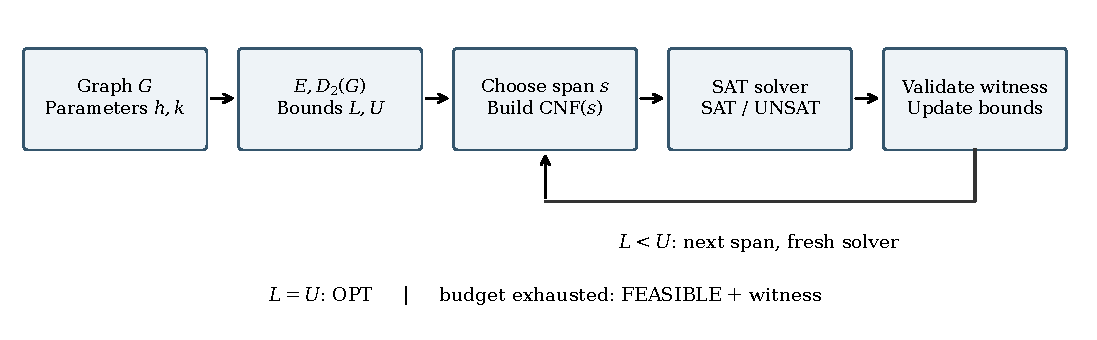
\includegraphics[width=\linewidth]{paper/generated/manuscript_figures/solver_pipeline.pdf}
\caption{SAT span-search pipeline.}
\label{fig:pipeline}
\tablenote{SAT pipeline for $L(h,k)$. A SAT result is decoded and validated
before decreasing the upper bound; UNSAT increases the lower bound. A timeout
retains the bounds and feasible incumbent and must not be treated as UNSAT.}
\end{figure}
\subsection{Bounds and search invariant}
For a graph with at least one edge, let $m=\min(h,k)$ and use
\[
 L=h+(\Delta(G)-1)m.
\]
Consider a maximum-degree vertex and its neighbors. Every pair in this set
has graph distance 1 or 2, so consecutive labels in sorted order differ
by at least $m$. At least one gap is incident to the central vertex's label
and has length at least $h$. Summing the $\Delta$ gaps gives the bound.
For $(2,1)$, this reduces to $\Delta+1$, as used in main\_r1.
An edgeless graph has span 0. The greedy algorithm excludes labels differing
by less than $h$ from already labeled neighbors and by less than $k$ from
already labeled vertices at distance exactly 2. Strict symmetry orders
are enabled only when $h,k>0$.

The greedy algorithm follows a fixed vertex order and chooses the smallest
nonnegative integer consistent with previously assigned labels. Let $U$
be the resulting span; the validator checks the labeling before it is used
as an incumbent. The invariant is
\[
 L\leq\lambda_{h,k}(G)\leq U,
\]
where the upper bound is always supported by an explicit labeling.

Linear search tests $s=U-1$. The revised hybrid search tests
$s=\lfloor(L+U)/2\rfloor$. On SAT, it decodes and normalizes the labeling
and reduces $U$ to the actual span. On UNSAT, it sets $L=s+1$.
It terminates with \OPT{} when $L=U$. A span with a known result need not
be solved again. Each trial constructs a CNF and a fresh solver; this
version does not use incremental SAT across spans.

\begin{proposition}
If the initial bounds are valid, the encoding is equivalent, and the
symmetry-breaking constraints preserve satisfiability, the search reports
\OPT{} only when the incumbent is optimal.
\end{proposition}
\begin{proof}
SAT provides a valid upper bound. UNSAT at $s$ excludes all spans at most
$s$ by monotonicity of the label domain. Both updates preserve the invariant.
When the bounds meet, they determine the optimum as the incumbent span.
\end{proof}
A timeout is not UNSAT and does not justify raising the lower bound.
If the budget expires with $L<U$, the algorithm returns \FEAS{} with its
incumbent. If the initial bounds already satisfy $L=U$, it may return
\OPT{} without calling SAT; variable and clause counts may then be absent.

\subsection{Validity of symmetry breaking}
Translation guarantees only that \emph{some vertex} receives label 0.
Fixing a chosen vertex $v_0$ to 0 requires an additional structural argument.
\begin{proposition}
If $G$ is vertex-transitive, imposing $f(v_0)=0$ preserves the optimal span
and the satisfiability of the decision problem with span at most $s$.
\end{proposition}
\begin{proof}
Normalize a valid labeling so that some vertex $w$ has label 0.
Vertex transitivity provides an automorphism mapping $v_0$ to $w$.
Composing the labeling with this automorphism preserves all distances
and assigns label 0 to $v_0$.
\end{proof}

For $C_n$, choose $t$ with $f(t)=\min_i f(i)$ and define
\[
 g(i)=f((i+t)\bmod n)-f(t).
\]
Rotation preserves distances and translation preserves label differences.
Thus $g$ is valid, $g(0)=0$, and its span equals that of $f$. The justification
is the cycle's rotational automorphism, not merely equality of vertex degrees.

In these experiments, root fixing is applied only to $C_n$. The general
proposition does not imply that the implementation fixes a root for every
vertex-transitive family. Other families use only the orders listed below.
Threshold variables for a fixed vertex need not be allocated; fixing one
vertex eliminates $s$ variables. Related constraints are evaluated using
constants and simplified before the solver is called. This reduces CNF
size through label fixing; adding an ordering inequality alone can increase
the clause count.

The same preprocessing is applied to both Baseline and Symmetry: removal
of tautologies and duplicates, followed by unit propagation to a fixed point.
For a unit clause $\ell$, all clauses containing $\ell$ are satisfied, and
$\neg\ell$ can be removed from the remaining clauses. The unit clause is
retained so that the decoder reconstructs the labels correctly. Each step
preserves logical equivalence over the original variables; deriving an empty
clause establishes UNSAT. Label fixing and bounds implied by ordering can
therefore simplify related constraints. Reported variable counts refer to
allocated variables, not those left unassigned after propagation; fixed-vertex
variables are eliminated during construction.

For a reflection exchanging two vertices $u,v$ that must have distinct labels,
solutions occur in pairs with opposite label orders. Imposing $f(u)<f(v)$
retains exactly one solution from each pair. This halves the \emph{number
of solutions} before combination with other symmetry constraints; it does
not imply a halving of clauses or runtime. The CNF is constructed by adding
constraints and simplifying, so its final size depends on the encoding
and the resulting deductions.

\begin{table}[H]
\centering\small
\begin{tabular}{p{0.25\linewidth}p{0.65\linewidth}}
\toprule
Family & Constraints in the revised implementation\\
\midrule
$C_n$ & $f(0)=0$ and $f(1)<f(n-1)$, using reflection about 0.\\
$K_n$ & Strict order by vertex index; no root fixing.\\
$Q_d$ & Order on neighbors $1,2,4,\ldots$ using coordinate permutations; no root fixing.\\
$C_n\mathbin{\square} C_m$ & Order only between $(1,0)$ and $(n-1,0)$; no root fixing.\\
$C_n\mathbin{\square} P_m$ & Order only between $(1,0)$ and $(n-1,0)$; no root fixing.\\
$GP(n,k)$ & Order only between outer neighbors $u_1,u_{n-1}$ using reflection $i\mapsto-i$.\\
$C_n\circ H$ & Order only between core neighbors 1 and $n-1$, reflecting the attached copies simultaneously.\\
$P_n\mathbin{\square} P_m$, $P_n\circ H$ & No family-specific constraints in this version.\\
\bottomrule
\end{tabular}
\caption{Symmetry breaking justified by explicit graph automorphisms.}
\end{table}
For orders between two neighbors, their labels are already required to differ
because their distance is at most 2. Reflection exchanges them while preserving
the other constraints. Equal degree alone does not justify interchangeability.
Structural metadata is used only when the vertex and edge sets are unchanged
from the constructor; a family name alone does not justify applying these
constraints to an arbitrary graph.

The implemented reflections are explicit. For Cartesian products with a
$C_n$ factor, $(i,j)\mapsto(-i\bmod n,j)$ exchanges the selected neighbors.
For $C_n\circ H$, reflection of core indices $i\mapsto-i\bmod n$ maps
copy $H_i$ to $H_{-i}$ while preserving internal indices. For Petersen graphs,
use $u_i\mapsto u_{-i}$ and $v_i\mapsto v_{-i}$; step-$k$ edges become
step-$-k$ edges, preserving the undirected edge set. The constructor uses
$u_i=i$ and $v_i=n+i$, consistent with the stored label indices.

\subsection{Post-hoc combinatorial certificates}
\label{sec:clique-method}
We also use an elementary packing bound to check stored solutions after
the experiments. This bound is separate from the degree bound used during
span search and is not claimed as a new general theorem.

\begin{proposition}
\label{prop:square-clique}
Let $G$ be a simple undirected graph, $h,k$ nonnegative integers, and
$Q\subseteq V(G)$ a set in which every two distinct vertices have distance
at most two in $G$. Then
\[
 \lambda_{h,k}(G)\geq \min(h,k)\max\{0,|Q|-1\}.
\]
If a valid labeling attains this bound, its span is optimal.
\end{proposition}
\begin{proof}
The claim is immediate for $|Q|\leq1$. Otherwise, sort the labels on $Q$
as $a_1\leq\cdots\leq a_q$. Each pair of vertices in $Q$ is subject to
separation $h$ or $k$, so $a_{i+1}-a_i\geq\min(h,k)$. Summing gives
$a_q-a_1\geq(q-1)\min(h,k)$, and the labeling's full span is at least
$a_q-a_1$. A feasible labeling attaining the lower bound supplies the
matching upper bound, proving optimality.
\end{proof}

Such a set $Q$ is a clique in $G^2$, where vertices are adjacent exactly
when their distance in $G$ is one or two. In the studied domain $h\geq k$,
the bound is $k(|Q|-1)$ for nonempty $Q$. Paths establishing distance two
may use vertices outside $Q$. No maximum-clique certificate is required:
membership of any proposed $Q$ suffices for the lower bound.
For the current small cohort, the postprocessor enumerates maximal cliques,
selects a largest one, and breaks ties lexicographically. Enumeration can
take exponential time; this is not a scalability claim or a change to
the timed SAT/ILP pipeline.

A separate verifier, using only the Python standard library, checks the
embedded graph, the complete labeling, all edge and distance-two label
constraints, clique membership, and both bounds. The exporter binds each
certificate to an audited experimental graph and saved witness; source
hashes and vertex indices are retained. This yields a direct combinatorial
optimality certificate when the bounds meet, without relying on SAT UNSAT
or ILP dual-bound claims. It does not certify optimality when the bounds
remain unequal.

\subsection{Time limits and solution validation}
A SAT conflict limit is not a wall-clock time limit \cite{pysat}. The revised
implementation runs span search in a child process, uses a monotonic clock,
and terminates the process when the remaining budget expires. This applies
to both Glucose and CaDiCaL without relying on backend-specific interruption
APIs. SAT runtime includes preprocessing, process startup, CNF construction,
search, validation, and process cleanup. Parent-process preprocessing is not
forcibly interrupted, so it and cleanup overhead may cause total runtime
to exceed the nominal limit. Unlimited calls execute directly.

ILP uses the backend's native time limit for optimization; reported runtime
also includes model construction and validation. These budget mechanisms
are not treated as identical when comparing SAT and ILP.
The validator checks the label domain, coverage of all vertices including
isolates, and the edge and distance-2 conditions. It verifies feasibility,
not UNSAT. Search history is likewise not an independently checkable UNSAT
certificate: this version does not export or verify DRAT/LRAT proofs.
